\documentclass[12pt]{article}
\usepackage{amsmath}
\usepackage{ amssymb }
\usepackage{tikz}
\usepackage{ textcomp }
\title{Course Recommendations \\Using the Social Network\\ {\Large \bf Midterm Report}}
\author{Wen-Hao Lee, Jamie Jackson, and Isaac Sheff}
\begin{document}
 \maketitle 
 

 

\newpage

\tableofcontents

\newpage

\section{Motivation}

Many businesses consider it a huge boon to be able to accurately predict which products a customer may want. They have worked so hard at this that they've actually generated hidden networks of users sorted and linked by their mutual interests. Traditionally, such networks are formed using learning algorithms that attempt to establish similarities between the preferences of sets of users. 

Consider, however, that the actual likes and dislikes of customers are highly affiliated with that user's social network.  A product enjoyed by a user's friends is probably more likely to be enjoyed by that user. In fact, traditionally, people seek out advice in such decisions from those closest to them on a social network. In fact, a study by Rashimi Sinha and Kirsten Swearingen at UC Berkely found that amongst books and movies, recommendations by friends were 30-40\% more likely to be ``Good" or ``Usefull" than traditional network recommendation systems [1].

Enter course recommendations. In a collegiate environment, especially at large institutions with extensive catalogues, students often rely on friends' recommendations to make important, periodic decisions: which courses to take. Students consider themselves more likely to enjoy courses their friends have enjoyed, with professors their friends have found effective. 

This provides an excellent testing ground for such a hybrid recommendation system, which would use traditional learning algorithms to suggest courses based on a student's past experience, compared with that of similar students, weighted accordingly for the distance of other students in the social network. 


\section{Prior Related Work}

Many traditional recommendation systems, such as Netflix, make use of Collaborative Filtering, in which a database of users' ratings of items is used to predict what a given user will rate an item based upon their past ratings [2]. A traditional, ``Memory-Based CF" system calculates a correlation factor between all users, and possibly all items, based on users existing rankings, and predicts rankings of a user's unranked items using the correlation weighted average of other users' rankings. It then recommends the top-ranked ones. There are a wide variety of alterations and improvements upon this simple idea for specific circumstances, computational constraints, and applications.

One such subset is the neighbor-based collaborative filtering model, in which a weighted average of rankings is taken only from a limited number of users most similar to the user in question. This is in some ways analogous to a limited ``friend" group on a social network, but the ``neighborhood" is made by the algorithm, not the user. 

Recommendation networks, however, do not take into account other factors in a user's life that can drive decision-making besides prior experience in the narrow field of whichever item type is being recommended. While many recommendation systems seek to account for such factors, generalization is extremely difficult. However, users seeking recommendations from friends receive an advantage over anonymous systems: trust. A test done at the Department of Computer Science and Engineering, Indian Institute of Technology, Delhi, found that users are more likely to receive better recommendations from other users they trust more, and that to a large extent, friendship on social networks (they used Orkut), mimics trust [3]. 

The idea of social-network based recommendations is not new. For example, the experimental service FilmTrust attempts to utilize Memory-Based CF calculating the similarity weighting between users as the trust between those users using the FOAF trust model [4].  Synclab Consulting's Hooks App for facebook recommends music found in the libraries of users' friends with many mutual songs in their playlists [5]. A study at the University of Illinois Champaign-Urbana found 95 \% of users on an experimental  social network-based news recommendation system to be ``somewhat to very useful" [6].  


As of yet, however, there appears to be a lack of course recommendation services making use of social networks, and a lack overall of social network ranking combined with collaborative filtering weighting users by both similarity and social distance. To study the feasibility of such a system, and to identify the appropriate weighting of social connections versus past user ranking similarity, we propose the creation of a facebook App, in which users rate and comment upon their past courses and professors, which will recommend additional courses and professors based upon the ratings of similar users, weighted by distance in the social network. By using Facebook, we gain a notable advantage over previous studes such as FilmTrust, which required users to build a trusted list inside its own framework. Facebook provides a similar system (friends, albeit without varying trust levels) ready-made. To begin with, we might use an algorithm which calculates the trust of various users via the FOAF model [4], and multiplies that by the measured similarity based upon past rankings (standard CF technique [2]), to determine the weight for each user. This algorithm will be adapted and conceivably radically changed to improve the system over the course of the project.  






\section{Objective}

\subsection{Facebook App}
The objective of this project shall be to produce a facebook app wherein users can specify their institute, classes they have taken, and the instructors for those classes. For each instructor and for each class users can rate quality as well as provide brief comments. The comments will be visible only to their friends. The ratings will be used in a hybridized CF recommendation system to predict what courses each user would also find to be of high quality, taking into account their past ratings compared with those of other users, as well as their social relations to those other users. 

To evaluate the effectiveness of a particular recommendation algorithm over the course of this project (since there will be insufficient time for users to take new classes, and respond with how well prediction matched reality), an assessment could be made of the average correlation between predicted ratings and actual ratings (average of ``how would this have been predicted to have been rated had I not rated it over how I did in fact rate it"). 

By testing which algorithm is best, in the optimal scenario, this app will identify what role, if any, social relations should play in course recommendations, which is likely to be similar to many other recommendation systems.

In order to acquire lots of users, the app will need to be sufficiently easy to use, and popularized through the developers' social contacts, contacting professors who might use the app for course feedback, and perhaps even advertising if necessary. Large institutes, with larger course catalogues and even larger student bodies, will likely make for better test data sources. 

\subsection{Science}

The worst case scenario is one in which insufficient user data can be acquired in time to analyze. Attempts shall be made to avoid this scenario through advertising and asking people to help us participate in an experiment through a wide variety of social channels, but ultimately it is possible that the experiment will be ignored. In this case, very limited conclusions can be drawn about the success or failure of cross-network data extraction. The week six evaluation period should catch on to this, and make any possible major project reevaluations. 

\section{Back End}

To host a Facebook application, a web server must provide reliable access for all users of that application to a web page. This web page is displayed inside Facebook's frame, but the actual access is directly from the user's browser to the host's web server. The web server itself as well as the javascript in the web page are granted access to Facebook's Graph API, with which they can access user information and send out wall posts, messages, and the like. Google's App Engine cloud service hosts Coursefinder. 

\subsection{Google App Engine}

Google's App Engine service was selected as Coursefinder's host because of its reliability, flexibility, and budget constraints. 

App Engine is a cloud service, meaning it is maintained as a distributed system across several large data centers owned and operated by Google. As such, the probability of any ``App" it runs becoming unavailable at any one time is extremely small. Additionally, the large number of available servers means that while intense average use may be equally costly, there is little danger of usage spikes overloading the server system, as opposed to a single server just for Coursefinder, which would likely have great difficulty if a large number of users decided to use the app at once. The combination of extremely low downtime and high spike tolerance make App Engine much more reliable than alternative, more traditional hosts, such as Caltech's notoriously poorly maintained UGCS, or a dedicated server. 

Several aspects of App Engine make it extremely flexible. For example, App Engine allows services written for the Java Runtime Environment and Python. Coursefinder is written in Python because, as a pure scripting language, and an incredibly flexible one, it allows great ease of manipulation and modularization of services. App Engine's support for Python made it a strong candidate. Additionally, because App Engine uses a noSQL hash table based database structure, data storage of any size is equally fast. In fact, aside from financial concerns over larger server usage, Coursefinder should be able to expand to an arbitrarily large set of institutions and users without speed or algorithmic problems. Furthermore, App Engine allows simultaneous deployment of different versions, allowing multiple tests to be run on the production server without interfering with regular service. This is extremely useful when, for example, different developers are simultaneously testing various new features and need to do so with real or large simulated data. 

As a small endeavor, Coursefinder has few resources with which to acquire, set up, run, and maintain a dedicated server facility. In effect, it requires a free service to run. While several are available, including Caltech's own UGCS, App Engine's free service offers more than Coursefinder is likely to require in the near future, and this on top of its other advantages made it the host of choice. 


There are some penalties for this. For example, while eventual consistency of data is assured, it is possible that reads from the database that take place shortly after writes to it will not pick up the new data. In the case of Coursefinder, this is not terribly troublesome, as it is not particulary important that data portrayed by ``up to the second." A more vexing problem is the noSQL database structure, which makes some forms of data relationships more difficult. Most notably, queries to the database cannot be nearly as complex, with serious problems concerning logical ``OR" operations. Again, these are usually minor problems for a system with fairly straightforward data storage and retrieval. 


 Coursefinder is hosted at http://courserecommendation.appspot.com.

\subsection{Django}


Django is a popular web development framework based in Python and built to run atop a variety of server setups. Django-nonrel, built for noSQL databases such as App Engine, was selected as a framework for Coursefinder because of its  portability and modularity. 

Django is built to be extremely portable. A running instance of Django, called a ``project," need only change a few settings variables to switch servers, databases, and even database structures. As a python framework, it is in no way platform specific, and it is entirely open source. Even within a project, the actual services offered, or ``apps," can be moved between projects with relative ease. One fortunate side effect is that it is extremely easy to run an instance of Django exactly as it would be run on App Engine on a local machine for testing purposes. It is equally easy to deploy to the production server. App Engine in particular has a number of features built in that are borrowed from Django, such as models and templates (and their associated syntax). Because of these, Django is an especially attractive option when developing on App Engine, but Coursefinder could relatively easily be modified to run on most any other server capable of running Django, should it at any time become a superior option to do so. 

Django is also extremely modular, which is useful when developing along separate tracks or as a team. It allows easier division of tasks, and overall more efficient rapid development. For example, rather than a traditional url to file hierarchy structure, Django replies to each HTTP request with the output of a function called a view, which is any function that takes in the HTTP request data and returns a web page. Which view is determined by a regular expression table. This means that it is very easy to add, subtract, and manipulate the ``structure" of urls independently from the construction of actual pages. It allows, for instance, the extremely simple ``/course/<course number here>/" urls, as opposed to some more complicated PHP scheme with GET url inputs. As another example, django's template system allows a well-designed seperation between content and formatting on the server side by allowing a view to fetch content, and pass it to a template, where the python content is easily inserted into the html template using ``{{ }}" tags, including basic flow control such as loops. This type of system allows, for instance, one developer to focus on content fetching and generation, while another focuses on formatting and presentation.


\subsection{Data Structure}

\begin{figure}[h]
  \caption{Data Structure}
  \centering
    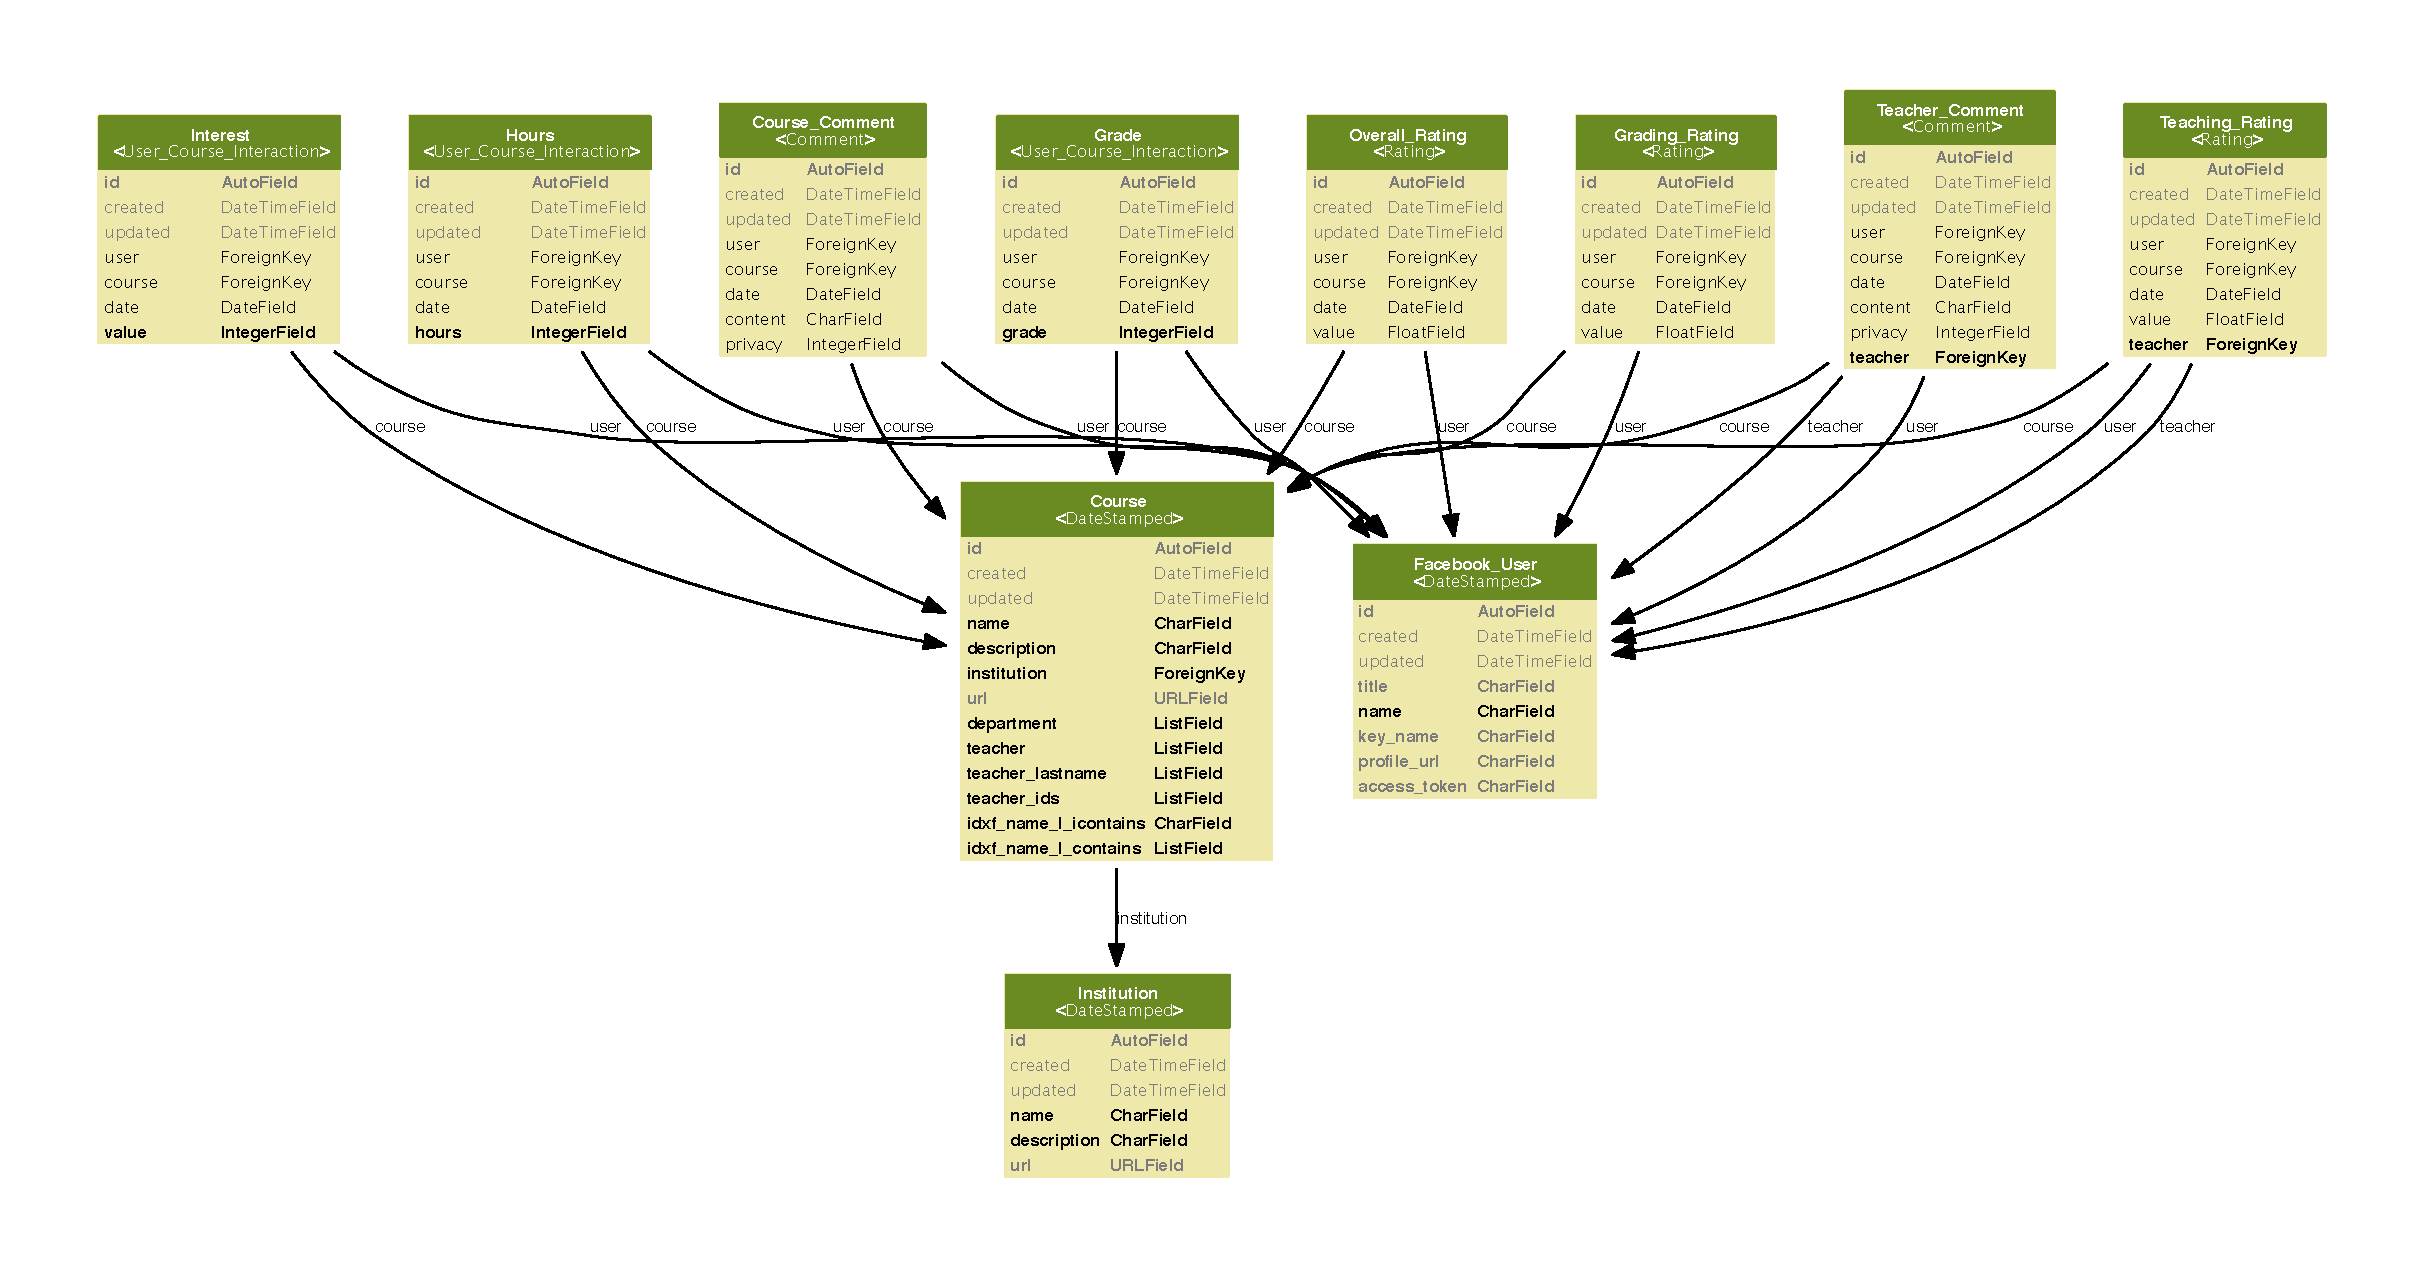
\includegraphics[width=6in]{data_structure.pdf}
    {\small \\Data structure UML for Coursefinder. Note that department is a list of string department abbreviations, and teacher\_ids is a list of valid ids of Facebook\_User objects. Also please note that the hideousness of UML is not my fault. }
\end{figure}


The data for Corusefinder is stored in the form of Django Models, for which a similar system is implemented natively for App Engine. Models, rather than the traditional way of thinking of data in tables, are simply objects of specific classes for which certain attributes, called fields, can be saved to the database and searched for in order to retrieve the object again. The types of fields used are CharField (string), DataTimeField, IntegerField, FloatField, URLField, ForeignKey (a link to another object stored in the database), and ListField, a field type specific to App Engine, which stores a list of any other kind of field. Notably, App Engine, as a noSQL database, cannot hand Many-to-Many fields, which store multiple other objects in the database. ListFields of ids, such as the ids of teachers for a course, are used instead. 

Django Models also support abstract inheritance. This allows abstract classes controlling common model features to be easily built upon or modified as may be needed. For example, there is an abstract Rating model, which allows the three different kinds of ratings (Teacher, Grading, and Overall), to only specify what differentiates them, and any common aspects of ratings to be changed easily. All models used in Coursefinder inherit the abstract model DateStamped, which ensures they all have a created DateTime storing the creation time of that object, and an updated DateTime, storing the last updated time of that object. 

The models, grouped by inheritance, employed to store the data for Coursefinder, are:

\subsubsection{DateStamped (Abstract)}
This is an abstract class (there are no objects with this class) designed so that classes which inherit it
	have creation and update timestamps.
\begin{itemize}
\item created: DateTimeField - date upon which this object was created
\item updated: DateTimeField - date upon which this object was last updated
\end{itemize}


\subsubsection{Facebook\_User (inherits DateStamped)}
	
	This is the model for a facebook user, as defined by Facebook's Python-SDK google appengine example
	
	Title is for use with teachers, and  the facebook-provided fields are optionally blank, so 
	Teachers can be created as Facebook\_Users without actually knowing their facebook info. 
	
	\begin{itemize}
	\item title : CharField, maximum length 100, optional, default ``": user's title 
	\item name : CharField, maximum length 100:  user's name 
	\item key\_name : CharField, maximum length 100, optional, default ``":  users's facebook ID
	\item profile\_url : CharField, maximum length 200, optional, default ``":  user's profile's URL
	\item access\_token : CharField, maximum length 255, optional, default ``":  user's oauth access token (facebook defined, changes)
\end{itemize}

\subsubsection{Institution (inherits DateStamped)}

	This model represents a university or college, or whatever else offers classes.
	
		\begin{itemize}
	\item name : CharField, maximum length 255, Insititution's Name
	\item description : CharField, maximum length 2023, Insititution's Description
	\item url = URLField, maximum length 255, optional, default ``": a url for this university. (optional)
\end{itemize}

\subsubsection{Course (inherits DateStamped)}

	This model represents a Course offered at a university of college.
	
	\begin{itemize}
	\item name : CharField, maximum length 255:  Course Name
	\item description : CharField, maximum length 1023:  Course Description
	\item institution = ForeignKey:  the institution offering this course
	\item url =URLField, maximum length 255, optional, default ``":  a url for this course. 
	\item department = ListField of CharField max length 100 chars each:  a list of this course's departments. 
	\item teacher = ListField of CharField max length 200 chars each
	\item teacher\_lastname=ListField of CharField max length 200 chars each
	\item teacher\_ids = ListField of IntegerField:  a list of ids of teacher models teaching this course
\end{itemize}

\subsubsection{User\_Course\_Interaction (Abstract, inherits DateStamped)}


	This is an abstract model, no objects actually have this class, designed to define the required fields for
	every other model which features a user and a course. (comments, ratings, etc . . . )
	
	\begin{itemize}
		\item user  : ForeignKey:  the user involved. 
		\item course  : ForeignKey:  the course involved
		\item date  : DateField, defaults to date created:  ideally the date the was taken.
\end{itemize}

\subsubsection{Hours (inherits User\_Course\_Interaction)}

	This is a model for recording the number of hours a user spent on a course
	
	\begin{itemize}
		\item hours  : IntegerField:  The number of hours the user spent on the course
\end{itemize}

\subsubsection{Grade (inherits User\_Course\_Interaction)}

	This is a model for recording the grade a user got in a course
	
	\begin{itemize}
		\item grade  : IntegerField: The grade a user got in a course 0=F, 1=D, 2=C, 3=B, 4=A
\end{itemize}


\subsubsection{Comment (Abstract, inherits User\_Course\_Interaction)}


	This is an abstract model, meaning you can't actually create and save these, designed to define the required fields for
	every other Comment based model
	
	\begin{itemize}
		\item content : CharField, maximum length 1023: Comment text
	\item privacy  : IntegerField:  Comment privacy rating. 0 for friends only, 1 for public
\end{itemize}


\subsubsection{Course\_Comment (inherits Comment)}

	A course comment, at the moment at least, has nothing more than a generic comment.
	


\subsubsection{Teacher\_Comment (inherits Comment)}
	
	A comment on a teacher, for a class.
	
	\begin{itemize}
		\item teacher  : ForeignKey:  the Teacher involved. 
\end{itemize}
	
\subsubsection{Interest (inherits User\_Course\_Interaction)}

	
	\begin{itemize}
		\item value  : IntegerField:  the interest tag is 0 (none) or 1 (interested in)
\end{itemize}


\subsubsection{Rating (Abstract, inherits User\_Course\_Interaction)}
	This is an abstract model, meaning you can't actually create and save these, designed to define the required fields for
	every other model for Rating Courses.
	
	\begin{itemize}
		\item value  : FloatField:  the value of a rating is a float. Let's standardize now. 0 is bad. 1 is good. Rate however you want.	
\end{itemize}

\subsubsection{Overall\_Rating (inherits Rating)}

	This is the overall rating for a course. It is just a rating. Nothing to add.
	


\subsubsection{Grading\_Rating (inherits Rating)}

	This is the Grading rating for a course. It is just a rating. Nothing to add.


\subsubsection{Teaching\_Rating (inherits Rating)}

	This is the teaching rating for a course, and a teacher. It is a rating, but now with both a course and a teacher.
	
	\begin{itemize}
		\item teacher  : ForeignKey:  the Teacher involved.
\end{itemize}







\section{Front End}

\subsection{Site Map}

\subsection{Layout}



\section{References}

\begin{enumerate}
\item Rashmi R. Sinha and Kirsten Swearingen. Comparing recommendations made by online systems and friends. In {\it DELOS Workshop: Personalisation and Recom- mender Systems in Digital Libraries}, 2001.

\item
Xiaoyuan Su and Taghi M. Khoshgoftaar, ``A Survey of Collaborative Filtering Techniques," {\it Advances in Artificial Intelligence}, vol. 2009, Article ID 421425, 19 pages, 2009.

\item
K. Sarda, P. Gupta, D. Mukherjee, S. Padhy, and H. Saran, ``A distributed trust-based recommendation system on social networks," in { \it HotWeb �08: Proc. of the 2nd IEEE Workshop on Hot Topics in Web Systems and Technologies}, 2008.

\item
Goldbeck, J. and Hendler, J.	2006.	FilmTrust: Movie recommendations using trust in Web-based
social networks. In { \it Proceedings of the IEEE Consumer Communications and Networking
Conference}. Las Vegas, NV.

\item
Synclab Consulting, "Hooks for Facebook."  {\it synclab consulting } 11 Mar. 2011, $<$http://www.synclab.com/hooks-for-facebook/$>$.

\item
M. Agrawal, M. Karimzadehgan, and C. Zhai. An online news recommender system for social networks. { \it SIGIR-SSM}, 2009.

\end{enumerate}
\end{document}